\chapter{Representación Vectorial de Palabras}

En esta sección se pretende realizar una recorrida por la literatura en el área de representación
vectorial de palabras, un tema que se ha ubicado en los últimos años en el centro de la escena en
muchas tareas de PLN\@. Se dará un pantallazo de qué entendemos por representaciones vectoriales, de
dónde surgen, y cuáles son los principales trabajos asociados a su desarrollo, mediante un
tratamiento más bien superficial que permita poner en perspectiva el trabajo que se realiza en el
presente proyecto de grado.


\section{Conceptos Básicos}

En los últimos años ha habido un importante cambio de paradigma en PLN, donde la mayor
investigación, y el mayor éxito, se ha obtenido con la aplicación de métodos de aprendizaje
automático para el tratamiento del lenguaje, en oposición a métodos basados en reglas.

Los métodos de aprendizaje automático son técnicas principalmente estadísticas que suelen tomar
vectores como entrada, por lo general reales. Dado que la unidad semántica básica del lenguaje
natural, las palabras\footnote{Se podrían considerar entidades aún más pequeñas como los morfemas
como unidad básica, pero el punto se mantiene.}, son entidades discretas y de gran cardinalidad, es
necesario realizar un mapeo entre estos dos espacios. Por esta razón es que existe un gran interés
en buscar y caracterizar mecanismos que permitan construir representaciones vectoriales para las
palabras del lenguaje.

Formalmente, si $V$ es el vocabulario con el que se está tratando en un contexto dado (por ejemplo,
$V = \{ \text{a}, \text{ábaco}, \text{abajo}, \ldots \}$), decimos que una función $F: V \to
\mathbb{R}^N$ induce una representación vectorial de dimensión $N$ para dicho vocabulario si le
asigna un vector de $\mathbb{R}^N$ a cada palabra de $V$ (e.g. $F(\text{a}) = (1.1, 0.9, \ldots,
0.2)$, $F(\text{ábaco}) = (2.3, 0.1, \ldots, 0.1)$).


La construcción de funciones $F$ que tengan buenas propiedades es un objeto de estudio muy
interesante y por lo tanto muy tratado, pues la performance de una gran cantidad de algoritmos de
PLN dependen directamente de la calidad de las mismas. Dependiendo el contexto en que se esté
trabajando, puede ser deseable requerirle a $F$ tener una algunas propiedades particulares:

\begin{itemize}

\item Puesto que los algoritmos de aprendizaje automático por lo general trabajan con vectores
reales continuos, suele ser un punto positivo que palabras que están relacionadas o que tienen
significados similares tengan asociados vectores que también sean similares en cierto nivel,
pudiendo explotar así la continuidad de los métodos utilizados.

Por ejemplo, imaginemos que se quiere entrenar un clasificador de tópico trivial utilizando
\textit{Support Vector Machines} para asociar a cada palabra del vocabulario una etiqueta indicando
el tema del que trata (supongamos \textit{Deportes} y \textit{No Deportes}). Será altamente deseable
que palabras que suelen aparecer en los mismos contextos estén cerca en el espacio vectorial
resultante, asociando vectores más cercanos entre sí a palabras como \textit{tenis}, \textit{fútbol}
y \textit{gol} que a palabras como \textit{gato} o \textit{comida}. Así, el algoritmo logrará
separar las palabras pertenecientes a ambas categorías más efectivamente.

\item Uno de los principales problemas de trabajar con el lenguaje natural es la dimensionalidad de
los vocabularios con los que se trata. Por esta razón, otro requerimiento interesante para las
representaciones vectoriales es que asocien a las palabras vectores de $\mathbb{R}^N$ donde $N \ll
|V|$, logrando así hacer tratables las dimensiones de las entradas.

\item Otra alternativa al punto anterior es generar representaciones de alta dimensionalidad pero
buscando que éstas sean dispersas: esto es, que los vectores asociados a las palabras tengan casi
todas sus entradas en cero. Esto hace más tratables a los vectores, puesto que permite el empleo de
técnicas de tratamiento de matrices dispersas, mejorando así la eficiencia desde el punto de vista
computacional y de almacenamiento.

\item Dado que se está embebiendo un espacio muy rico en estructura, tanto desde el punto de vista
semántico como sintáctico, es de particular interés lograr mantener dicha estructura en el espacio
de destino: esto es, obtener una representación que exhiba regularidades lingüísticas en alguna
medida.

Por ejemplo, sería satisfactorio que la relación que existe entre el par de palabras \textit{correr}
y \textit{corriendo} (esto es, el gerundio) pudiera ser capturada matemáticamente, y que fuera el
mismo que presentan las palabras \textit{jugar} y \textit{jugando}. O, desde un punto de vista
semántico, que el par de palabras \textit{frío} y \textit{calor} presente las mismas propiedades que
\textit{alto} y \textit{bajo}.

\end{itemize}


Desde las distintas áreas del PLN se han desarrollado una gran cantidad de métodos para la
construcción de representaciones vectoriales que cumplan con algunas de las propiedades anteriores,
donde el elemento común suele ser la utilización de grandes cantidades de texto a partir del cuál
inferir buenas representaciones. Por esta razón, las representaciones vectoriales suelen recibir
diversos nombres, dependiendo de la literatura consultada.

Uno de los enfoques más tradicionales recibe el nombre de \textit{modelos semánticos
distribucionales} (o DSMs por su sigla en inglés) los cuales, inspirados en el campo de la semántica
estadística y la hipótesis distribucional~\cite{Harris1954}, hacen uso de estadísticas globales
derivadas de un corpus de texto para aprender representaciones que capturen la semántica de las
palabras. En este grupo de técnicas se puede encontrar el modelo LSA~\cite{Dumais1988,
Deerwester1990}, junto con sus principales variantes, y el modelo HAL~\cite{Lund1995,
LundBurgess1996}.

El otro gran enfoque en la construcción de representaciones vectoriales es el proveniente de la
comunidad de modelado de lenguaje mediante redes neuronales. Estos son métodos predictivos que
utilizan información local para construir modelos de lenguaje a partir de redes
neuronales~\cite{Bengio2003} y redes neuronales recurrentes~\cite{Mikolov2010}. Como efecto
secundario de estos algoritmos se obtienen también vectores para las palabras del lenguaje, las
cuales suelen denominarse \textit{vectores o modelos neuronales}, o \textit{embeddings} de palabras.

Otros nombres utilizados incluyen \textit{representaciones vectoriales continuas}, \textit{espacios
de palabras semánticos}, o simplemente \textit{vectores de palabras}.

Destacamos también la existencia de técnicas basadas en métodos aglomerativos para la construcción
de representaciones vectoriales más compactas. Un ejemplo son los métodos basados en el algoritmo de
Brown~\cite{Brown1992} (denominados \textit{Brown Clusters}): bajo este esquema, se realiza un
\textit{clustering} jerárquico de palabras utilizando estadísticas de los bigramas del corpus, tales
como su información mutua, y se construye un código que busca minimizar el largo de las
representaciones para grupos de palabras semánticamente relacionadas. También existen diferentes
técnicas que se basan en modelos ocultos de Markov~\cite{LiMcCallum2005} o en
K-means~\cite{LinWu2009}. Sin embargo, dado que estos modelos no han tenido los mejores resultados
en la literatura, y que tienen la desventaja de no producir representaciones continuas, limitaremos
nuestro estudio en el presente proyecto a los dos enfoques anteriormente presentados.


Vectores de palabras obtenidos con distintos mecanismos han sido utilizados exitosamente para una
gran cantidad de tareas de PLN, en especial en los últimos años, donde se han superado resultados
del estado del arte mediante la combinación de los mismos con aprendizaje profundo (o \textit{deep
learning}, como es conocido en la literatura). Mencionamos a continuación algunos de los principales
resultados.

\begin{itemize}

\item En~\cite{Socher2011a, Socher2013a}, se utilizan vectores basados en modelos neuronales para
realizar análisis de sentimiento en críticas de películas a nivel de árboles de parsing, superando
levemente los resultados obtenidos anteriormente.

\item En~\cite{CollobertWeston2008, CollobertWeston2011}, los autores plantean un nuevo esquema para
resolver problemas de PLN utilizando redes neuronales convolucionales cuya única entrada son
vectores de palabras, logrando resultados muy cercanos al estado del arte en tareas como \textit{POS
tagging} (etiquetado de categorías gramaticales), etiquetado de roles semánticos, y reconocimiento
de entidades con nombre.

\item En~\cite{Turian2010}, se mejoran los resultados obtenidos en reconocimiento de entidades con
nombre y en \textit{chunking} al agregar vectores de palabras como \textit{features} en un algoritmo
de CRF (campos aleatorios condicionales).

\item En~\cite{Socher2011b}, mediante la utilización de representaciones vectoriales y de
\textit{autoencoders}, se mejora el estado del arte en materia de detección de parafraseo en textos
cortos.

\item En~\cite{Mikolov2007}, el autor entrena una red neuronal recursiva utilizando como única
entrada vectores de palabras para generar un modelo de lenguaje para el checo, que posteriormente es
utilizado para reconocimiento automático de habla.

\item En~\cite{Socher2013b}, se generan vectores de palabras bilingües, donde se aprenden
representaciones para dos lenguajes de manera simultánea, obteniendo buenos resultados en traducción
automática de frases cortas.

\end{itemize}


En las siguientes secciones presentaremos una descripción más detalladas de los principales enfoques
para la construcción de representaciones vectoriales, llegando así a los métodos del estado del arte
en el área.


\section{Modelos Estadísticos}

Los modelos estadísticos se originan en el área de la lingüística computacional, basándose en
estudios teóricos de semántica distribucional de lingüistas como Zellig Harris, con su
\textit{hipótesis distribucional}~\cite{Harris1954}, y John Firth, con su noción de \textit{contexto de
situación}~\cite{Firth1957}, haciendo referencia a la dependencia que tiene el significado de las
palabras del contexto en el que ocurren (o, como lo plantea Firth, \textit{Conocerás una palabra por
la compañía que mantiene}). El hecho de que surjan hace tantos años dotan al área de una literatura
muy rica y extensa. A continuación daremos una breve reseña, recorriendo los resultados más
significativos.

La idea principal detrás de estos modelos es, pues, describir a las palabras del vocabulario según
el contexto en el que estas ocurren en un determinado corpus de texto utilizado para la construcción
de las representaciones. Con este fin, se construye un vector $v \in \mathbb{R}^N$ que captura, de
alguna manera, información acerca del contexto donde aparece la palabra.

Qué es considerado como el contexto de una palabra es una decisión propia de cada método; para un elemento
lingüístico particular, se podría considerar la pertenencia a una región de texto dado (e.g.\ la
pertenencia a una oración, un párrafo, o hasta un documento entero), o se puede considerar
definiciones que sean independientes de la estructura, considerando la relación con otros elementos
lingüísticos (e.g.\ la cantidad de \textit{coocurrencias} con otra palabra).

Para el punto anterior, también es importante definir qué \textit{métrica de asociación} se estará
usando respecto al contexto elegido: el caso más básico es contar la cantidad de ocurrencias de la
palabra en dicho contexto, pero existen técnicas que capturan mejor esta relación.

Otro punto importante a considerar es que la cantidad de contextos que se consideran puede ser muy
elevada: en el caso de coocurrencias con elementos lingüísticos, el vector asociado a un contexto
tendrá un tamaño del orden de $|V|$ elementos (donde $V$ es el vocabulario), mientras que si se
consideran regiones de texto se estará tratando con dimensiones aun mayores. Por esta razón, es
necesario evaluar el uso de técnicas de reducción de dimensionalidad, o al menos métricas de
asociación que generen representaciones dispersas que hagan al resultado tratable computacionalmente
(esto es, vectores con muchos ceros).

Por último, cómo utilizar la representación final obtenida y cómo medir la similitud entre dos
palabras es un tema no menor a resolver, que dependerá de la aplicación final de los vectores. Por
ejemplo, cuando se trata con representaciones dispersas, utilizar la distancia coseno en lugar de la
euclídea puede ser más eficiente (en especial cuando se normalizan los vectores) porque permite
descartar las componentes nulas en los cálculos.

Resumiendo, a la hora de construir un modelo estadístico para la representación vectorial de
palabras, es necesario tomar las siguientes decisiones:

\begin{itemize}

\item \textbf{Tipo de contexto}: utilizar regiones de texto o relaciones con otros elementos
lingüísticos.

\item \textbf{Forma que tendrá este contexto}: la forma que tendrán las regiones de texto
consideradas o la ventana de coocurrencia con los elementos lingüísticos.

\item \textbf{Métrica de asociación}: cómo se medirá la relación de una palabra con su contexto.

\item \textbf{Reducción de dimensionalidad}: cómo se manejará el tamaño elevado de las
representaciones obtenidas.

\item \textbf{Integración}: cómo utilizar los vectores en la tarea en la que se trabaja. Este punto
no es particular a los modelos estadísticos, pero es bueno resaltarlo, pues es de suma
importancia. Podría involucrar, por ejemplo, determinar cómo medir la similitud entre dos palabras
si se van a utilizar directamente o, si servirán como \textit{features} en un algoritmo de
aprendizaje automático, cómo encajarlos en esta maquinaria más grande.

\end{itemize}

Siguiendo los puntos anteriores, un modelo estadístico se podría formalizar de la siguiente manera:

\begin{itemize}

\item Un vocabulario $V$, conjunto de palabras que se considerarán. $V$ podría formarse con las palabras
que están presentes en el corpus, por ejemplo.

\item Un conjunto de contextos $C$, que captura las decisiones respecto al tipo y forma de los
contextos a utilizar. $C$ podría ser una lista de documentos (donde $c_1 \in C$ corresponde al
primer documento, $c_2 \in C$ al segundo, etc.), o un conjunto de elementos lingüísticos con los que
se medirá la coocurrencia (podrían ser las palabras de $V$, por ejemplo).

\item Una matriz de asociación $A \in \mathcal{M}_{|V| \times |C|}(\mathbb{R})$, que captura la
métrica de asociación entre el vocabulario y el contexto. Si $f: V \times C \to \mathbb{R}$ es la
métrica de asociación entre la palabra y su contexto, entonces $A = (a_{ij}) = f(v_i, c_j)$.

\item Una transformación de reducción de dimensionalidad $R: \mathcal{M}_{|V| \times
|C|}(\mathbb{R}) \to \mathcal{M}_{|V| \times d}(\mathbb{R})$, donde $d$ es la dimensión de los
vectores resultantes asociados a las palabras de $V$. $R$ podría eventualmente ser la identidad (y
$d = |C|$), o podría ser la aplicación de técnicas como SVD\@.

\item La matriz de traducción $T$, resultado de aplicarle $R$ a la matriz de asociación $A$ (i.e. $T
= R(A)$), es la matriz utilizada para ir de una palabra codificada bajo un esquema \textit{one-hot}
al espacio de vectores asociado al vocabulario $V$: esto es, las filas de la matriz corresponden a
los vectores de las palabras de $V$.

\end{itemize}

Cabe aclarar que la formalización recién presentado es más bien de carácter general y de ningún modo
exhaustiva: mientras que la mayoría de de los modelos estadísticos siguen el esquema anterior, hay
variantes que no encajan a la perfección pero no por eso se los deja de considerar modelos
estadísticos.


Como se mencionó anteriormente, los modelos estadísticos tienen una larga historia, principalmente
en las áreas de recuperación de información (IR, por sus siglas en inglés) y representaciones
vectoriales semánticas.

Uno de los primeros trabajos en el área fue el modelo de análisis latente semántico (LSA) propuesto
en~\cite{Dumais1988}, también llamado indizado latente semántico (o LSI, en especial en el área de
IR). Siguiendo un modelo basado en resultados de la psicología, los autores proponen utilizar
documentos enteros como contextos, y contar la cantidad de veces que una palabra dada ocurre en un
documento como métrica de asociación. Una vez construida esta matriz, los autores proponen utilizar
una descomposición en valores singulares (SVD, por sus siglas en inglés) de dicha matriz,
truncándola a los $d$ valores singulares más grande, donde $d$ varía dependiendo del caso (los
autores utilizan $100$ en algunos casos, $200$ en otro).

En~\cite{Deerwester1990}, los autores continúan con la técnica anterior, pero variando la métrica de
asociación: consiguen un mejor resultado utilizando TF-IDF en lugar de las frecuencias absolutas
para las coocurrencias. El objetivo principal de LSI es la recuperación de documentos basados en una
consulta, donde una palabra dada se proyecta al espacio de dimensión reducida y se devuelven los
documentos más cercanos en dicho espacio.

En~\cite{LandauerDumais1997} los autores profundizan y formalizan los anteriores modelos, incluso
planteando LSA como un modelo de adquisición del lenguaje en humanos. Además proponen la utilización
la entropía (de teoría de la información) como métrica de asociación alternativa, mejorando los
resultados obtenidos en tareas de similitud de palabras.

Continuando con estas ideas,~\cite{Hoffman1999} propone una variante al algoritmo anterior,
denominado LSI probabilístico (o pLSI, pLSA). Plantea formalmente la noción de variables latentes,
denominadas tópicos, relacionadas a documentos y palabras. Bajo este esquema, en lugar de utilizar
SVD para reducir la dimensionalidad, los autores plantean fijar a priori la cantidad de tópicos, que
corresponde a la dimensión $d$ resultante de los vectores, y luego expresar cada documento como una
combinación (denominada \textit{mixture}) de dichos tópicos. Cada palabra tiene una cierta
probabilidad de utilizarse en un tópico dado, y todos los parámetros se ajustan mediante un
algoritmo de maximización de la esperanza.

Otra variante al último algoritmo es la propuesta en~\cite{Blei2003}, donde los autores plantean un
modelo generativo denominado LDA (asignación de Dirichlet latente) que sigue un esquema de pLSI
donde la distribución de fondo para los tópicos se asume que sigue una distribución de Dirichlet.


Los anteriores modelos emplearon contextos basados en documentos. Otra corriente paralela fue
propuesta en~\cite{Lund1995, LundBurgess1996}, denominada análogo en el hiperespacio para el
lenguaje (o HAL). En esta propuesta, los contextos son ventanas de largo fijo alrededor de cada
palabra. Esto es, se construye una matriz de tamaño $|V| \times |V|$, y en la entrada $(v_i, v_j)$
se acumula el resultado la métrica de asociación $f(v_i, v_j)$ por cada vez que $v_j$ aparece en una
ventana alrededor de un $v_i$.

En el planteo original, los autores proponen formar una matriz de $|V| \times 2|V|$, y consideran
una ventana de largo 10 a la izquierda y otra a la derecha de la palabra central ($v_i$, en el caso
anterior). La métrica de asociación utilizada es el inverso de la distancia entre ambas palabras
(donde la palabra más cercana toma el valor $1$, mientras que el más lejano $1/10$).

Para la reducción de la dimensionalidad, los autores se quedan con las 200 componentes con más
varianza, bajo la observación que para la mayoría de las palabras la varianza es casi nula. Esto
corresponde a quedarse con las 200 palabras que presentan mayor varianza en sus entradas.
En~\cite{VayrynenHonkela2004} se obtienen mejores resultados (aunque a un costo computacional mayor)
realizando un análisis de componentes independientes (ICA) para reducir la dimensionalidad.


Distintas alternativas se han empleado también para la reducción de dimensionalidad, además de SVD,
ICA o las técnicas probabilísticas de pLSA\@. Una de las que mayor éxito ha tenido fue el indizado
aleatorio (también conocido como \textit{random indexing}, \textit{random mapping}, o \textit{random
projection}), propuesto en~\cite{Kaski1998}, el cual propone quedarse con $d$ dimensiones elegidas
aleatoriamente de la matriz de coocurrencias. Esta técnica se basa en el lema de
Johnson-Linderstrauss, que plantea que las distancias entre los vectores de palabras entre el
espacio original y el reducido se preservarán casi completamente, siempre y cuando el valor de $d$
sea suficientemente grande. En~\cite{Sahlgren2001}, se emplea esta técnica en lugar de SVD siguiendo
un esquema HAL\@.


En cuanto a métricas de asociación, mucho trabajo se ha centrado alrededor de la información mutua
puntual entre dos palabras (o PMI, ecuación detallada en~\ref{eqn:pmi}). Esta medida fue propuesta
inicialmente en~\cite{ChurchHanks1990} y busca modelar correctamente nociones de asociatividad entre
palabras del lenguaje: el hecho de que frases como \textit{cuesta arriba} son más comunes que
\textit{cuesta derecha}. El trabajo inicial de los autores no estuvo relacionado a representaciones
vectoriales, pero fue tomado más adelante por~\cite{Turney2001} con ese fin. En dicho trabajo se
presenta un algoritmo que usa PMI como medida de asociatividad, y compara los resultados con LSA\@.

\begin{figure}[h]
  \[
    pmi(w_1, w_2) = \log \frac{P(w_1, w_2)}{P(w_1) P(w_2)}
  \]
  \caption{PMI entre las palabras $w_1$ y $w_2$. $P(w_1, w_2)$ es la probabilidad de que coocurran
en un contexto (definido a priori). Las probabilidades se pueden estimar a partir de un corpus.}
  \label{eqn:pmi}
\end{figure}

De todos modos, no es hasta~\cite{BullinariaLevy2007} que se utiliza dicha métrica para la
construcción explícita de modelos vectoriales del lenguaje. En este trabajo los autores hacen una
evaluación sistemática de distintos parámetros para la construcción de vectores basándose en un
esquema HAL\@. Una de los principales aportes fue la introducción de la PMI positiva (PPMI), igual a
la PMI pero donde los valores negativos se sustituyen por cero. La intuición detrás de este cambio,
plantean los autores, es que los valores negativos implican que el par de palabras tiene menos
coocurrencias de lo esperado, punto que se podría dar por, por ejemplo, un corpus de tamaño
insuficiente o ruidoso. Otra ventaja de esta métrica es que la matriz de asociación resultante es
dispersa, lo que ayuda a que su cálculo sea manejable computacionalmente y a que la reducción de
dimensionalidad no sea imprescindible.

Además de métricas de asociación, los autores realizan pruebas con la dimensionalidad de los
vectores resultantes (quedándose únicamente con las $d$ palabras de mayor frecuencia), con el tamaño
del corpus utilizado para tomar las estadísticas, y con el tamaño de la ventana empleada. Llegan
finalmente a que, en todos los casos, los mejores resultados se obtienen con la métrica PPMI, en
especial cuando los tamaños de las ventanas son muy chicos (1 ó 2 a ambos lados de la palabra). En
cuanto al corpus y la dimensionalidad, cuanto mayor mejor, aunque está claro que esto afectará muy
negativamente a la eficiencia computacional.

Esta línea de investigación se continúa en~\cite{BullinariaLevy2012}, donde se evalúa también la
utilización de técnicas de reducción de dimensionalidad. Los autores muestran que los resultados se
pueden mejorar significativamente aplicando SVD y truncando a los $d$ valores singulares más grandes
(donde $d$ varía según el problema objetivo, pero suele estar cerca de $d = 1000$).  Además, logran
mejorar aún más los resultados mediante una variante de SVD propuesta por~\cite{Caron2001}, donde
la matriz de valores singulares se eleva a un exponente $P$, nivelando dichos valores para quitarles
peso a los más grandes.


El estado del arte en modelos estadísticos sigue principalmente el esquema recién planteado, pero
introduciendo algunas variantes adicionales inspiradas en los modelos neuronales:
en~\cite{Levy2015}, los autores utilizan distintas heurísticas para preprocesar el corpus con el que
se entrena el modelo (como realizar un \textit{subsampling} de palabras muy frecuentes, normalizar
los vectores resultantes, o eliminar palabras raras del vocabulario), logrando así mejorar
significativamente la calidad de las representaciones obtenidas.


\section{Modelos Neuronales}

La representación distribuida de conceptos mediante el uso de redes neuronales fue presentada
inicialmente en~\cite{Hinton1986}. En este artículo, el autor plantea la idea de usar los pesos de
las capas internas de redes neuronales básicas como la representación de un concepto particular en
un espacio continuo. Esta idea fue también propuesta por Rumelhart en~\cite{Rumelhart1986}, donde se
realiza una exposición más completa del mecanismo.

Aunque Hinton y Rumelhart plantearon inicialmente la idea de aprender conceptos abstractos (como
relaciones familiares), la técnica no tardó en extenderse al lenguaje natural. En 1990,
Elman~\cite{Elman1990} aplica redes neuronales recursivas básicas (denominadas \textit{Elman
networks}, utilizadas para realizar modelado a través del tiempo) a la tarea de predicción de
oraciones y utiliza los pesos internos aprendidos por la red como representación de las palabras. En
las pruebas que llega a realizar el autor (rudimentarias, debido al poder de cómputo disponible en
la época), consigue resultados prometedores, donde la representación de palabras como \textit{girl}
y \textit{woman} quedan más próximas que palabras como \textit{cat} y \textit{mouse}. Estos
resultados comparten ideas de la hipótesis distribucional, aunque su autor no hace mención explícita
a la misma.

De todos modos, debido a la dificultad de entrenar dichas redes neuronales, la técnica quedó en
desuso por varios años más.

No fue hasta 2003 donde Bengio presenta en~\cite{Bengio2003} una alternativa competitiva al modelado
de lenguaje a través de n-gramas\footnote{Los modelos de n-gramas, o modelos estadísticos, buscan
caracterizar al lenguaje en base a la probabilidad de secuencias cortas de palabras denominadas
n-gramas, y fueron el estado del arte hasta la década pasada.} mediante la utilización de redes
neuronales. El autor plantea la idea de utilizar el espacio real para modelar el lenguaje, con el
fin de explotar la continuidad local para obtener una mejor generalización, cualidad que carecen los
modelos estadísticos basados en espacios discretos. Por ejemplo, en un modelo de lenguaje basado en
unigramas o bigramas, la verosimilitud de la frase ``el gato corre'' es completamente independiente
de la de la frase ``el perro corre'', y la aparición de la primera en el corpus no elevará la
probabilidad de la segunda. Esto implica además que es necesaria una mayor cantidad de parámetros
para la estimación: una probabilidad de ocurrencia por n-grama. Otro punto positivo es que, al
requerir menos parámetros, es posible utilizar contextos más grandes: mientras que el estado del
arte en modelos estadísticos utilizan 3 ó 4 palabras, los modelos continuos llegan a utilizar hasta
10 ó 15.

La idea principal detrás del modelado continuo de lenguaje es distribuir la densidad de probabilidad de
la siguiente palabra (dada una secuencia de palabras inicial) de forma más inteligente: mientras que
los modelos estadísticos la distribuyen uniformemente alrededor de cada combinación de n-gramas
(e.g.\ de igual manera para ``el gato árbol'' que para ``el gato camina'', dada la frase ``el gato
corre''), los modelos continuos buscan que palabras relacionadas reciban más masa de probabilidad
que las que no están relacionadas.

En su artículo, Bengio presenta un esquema distinto al usual para entrenar el modelo de lenguaje:
plantea una arquitectura que consta de vectores continuos de palabras y una función paramétrica
definida sobre dicho espacio de vectores, el cual modela la probabilidad de la siguiente palabra
dada una ventana de $N$ palabras precedentes. El autor utiliza una red neuronal para modelar la
probabilidad, pero deja abierta la posibilidad de usar otros modelos, como modelos de combinación gaussiana
(o \textit{gaussian mixture models}). Bajo esta arquitectura, tanto los vectores de palabras como la
función de probabilidad son aprendidas en simultáneo, utilizando un corpus de gran tamaño como
entrada al algoritmo.

La principal innovación de este artículo fue la separación de los vectores de palabras y la función
de modelado de la probabilidad; de hecho, en~\cite{MiikkulainenDyer1991} ya se habían utilizado
redes neuronales para el modelado de lenguaje. El esquema de Bengio logra así mejorar
significativamente el estado del arte en materia de modelado de lenguaje, en especial a lo que
respecta a la eficiencia (comparando con otros modelos basados en redes neuronales), desatando una
nueva ola de investigación en el área, tanto en cuanto al modelado mediante redes neuronales como a
la utilización de los vectores de palabras que deja como resultado adicional el algoritmo.


A partir de este artículo, surgen también variantes de la arquitectura anteriormente
descrita. En~\cite{Mikolov2007, Mikolov2009} Mikolov presenta una arquitectura alternativa, donde se
aprende primero por separado las representaciones vectoriales utilizando un método no supervisado
basado en recorrer bigramas en un corpus de texto; esto es, utiliza una ventana de largo dos, si se
sigue el esquema anterior, pero los aprende independientemente del modelo de lenguaje. Luego estos
vectores son utilizados para entrenar una red neuronal que modela el lenguaje. Bengio en su artículo
original presentó una variante similar a esta, donde propone incluso la idea de utilizar vectores de
LSA fijos, en lugar de entrenarlos junto a la red, pero obtuvo resultados inferiores.

Otra variante propuesta por Mikolov~\cite{Mikolov2010, Mikolov2011a, Mikolov2011b, Mikolov2011c}
fue, en lugar de utilizar una ventana de largo fijo y una red neuronal estándar, utilizar una red
neuronal recursiva simple para modelar el lenguaje. Esta arquitectura es similar a las \textit{Elman
networks}, pero el autor obtiene mejores resultados por utilizar técnicas de entrenamiento modernas
que atenúan los problemas usuales de entrenar redes neuronales recursivas (RNNs). Como derivado de
este modelo también se generan representaciones vectoriales. El autor incluso ofrece una herramienta
de código abierto (\textit{RNN toolkit}) para la creación de modelos de lenguaje que sigan esta
arquitectura, pudiendo obtener tanto los vectores como el modelo de lenguaje~\cite{Mikolov2011c}.


Por otro lado, la aparición de estos modelos generó gran interés en el uso de representaciones
distribucionales para distintas tareas de PLN, más allá del modelado de
lenguaje. En~\cite{CollobertWeston2008}, los autores presentan una nueva arquitectura genérica para
la resolución de problemas de PLN utilizando exclusivamente aprendizaje profundo (esto es, sin
ingeniería de features), inspirados por el esquema propuesto por Bengio. Esta propuesta se basa en
la noción de aprendizaje por transferencia (conocido como \textit{transfer learning} o
\textit{multi-task learning}), donde se entrena un modelo para resolver más de una tarea a la vez,
con el objetivo de que el conocimiento que adquiere en una tarea pueda ser de utilidad en otra.

Con este fin, entrenan primero un modelo de lenguaje siguiendo la arquitectura de Bengio y luego,
con los vectores resultantes, entrenan en simultáneo cuatro redes neuronales para distintas tareas
(\textit{POS tagging}, \textit{chunking}, etiquetado de roles semánticos, etiquetado de entidades
con nombre), propagando los errores hasta los vectores. Logran así mejorar el estado del arte en
todas las tareas que prueban, donde destacan particularmente los resultados de SRL por considerarla
la tarea más compleja. El resultado de este trabajo es de gran importancia, porque plantea la
utilización de representaciones vectoriales como una nueva alternativa para la resolución de
problemas y muestra que es una técnica competitiva con las técnicas existentes.


Con este nuevo auge de aplicaciones de las representaciones, se comienza también a buscar mejorar
la eficiencia en la generación de vectores de palabras independientemente del modelado de
lenguaje. En~\cite{MnihHinton2007}, los autores proponen variantes a la arquitectura de Bengio que
buscan ser mejores desde el punto de vista computacional. De las cuatro variantes que proponen, una
de ellas, un modelo \textit{log-bilinear} (LBL), consigue incluso mejores resultados en la tarea de
modelado de lenguaje. Esta técnica es luego extendida a una versión jerárquica y más rápida
denominada HLBL en~\cite{MnihHinton2009}, haciendo uso de una versión jerárquica de la función
\textit{softmax}, propuesta por Bengio en~\cite{MorinBengio2005}.


En~\cite{Mikolov2013a}, Mikolov muestra que los vectores generados por una RNN (en particular, por
una RNN entrenada utilizando su \textit{RNN toolkit}) presentan regularidades lingüísticas muy
interesantes: además de los vectores ser muy buenos en tareas de similitud y relación entre
palabras\footnote{Por ejemplo, decidir si una palabra es sustituible por otra en un contexto
dado. En las siguientes secciones se dará una descripción más detallada de estas tareas.}, éstos
logran capturar relaciones sintácticas y semánticas a través de vectores específicos a cada
relación. El autor ejemplifica este fenómeno a través de la resolución de analogías\footnote{Por
ejemplo, vectores que capturen la relación de género entre dos palabras, de modo que a partir de los
vectores de \textit{hombre}, \textit{mujer} y \textit{rey} se pueda recuperar la palabra
\textit{reina}. Más adelante se entrará en mayor detalle.}, y construye un conjunto de pruebas
compuesto por analogías sintácticas.

Utilizando dicho conjunto, compara el rendimiento en esta tarea con sus vectores, con vectores
basados en modelos estadísticos (aunque no hace una comparación exhaustiva, por lo que no obtiene
buenos resultados), con los vectores generados por Collobert y Weston~\cite{CollobertWeston2008}, y
por los generados por Mnih y Hinton (HLBL~\cite{MnihHinton2009}), obteniendo los mejores resultados
con los propios y los HLBL\@.

Los resultados obtenidos en el anterior artículo motivaron la propuesta, por parte de Mikolov
en~\cite{Mikolov2013b}, de dos arquitecturas novedosas para la construcción de vectores, centrada en
la tarea de analogías y en mejorar la eficiencia computacional. En estas arquitecturas se deja de
lado la RNN y el modelado de lenguaje, y se centra exclusivamente en la construcción de vectores.

Ambos esquemas propuestos se basan en definir una ventana de largo fijo, simétrica alrededor de una
palabra central, y plantear un problema de optimización basado en predecir la palabra central dado
el contexto o vice versa. El primer caso recibe el nombre de \textit{Continuous Bag-of-words} (o
CBOW, esquematizado en~\ref{fig:cbow}), mientras que el segundo recibe el nombre de
\textit{Skipgram} (o SG, esquematizado en~\ref{fig:sg}).

\begin{figure}[h]
  \centering

  \begin{subfigure}[b]{0.45\textwidth}
    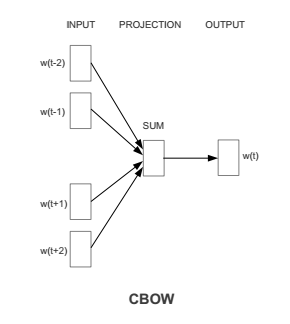
\includegraphics[width=\textwidth]{images/fig-2-cbow}
    \caption{Modelo Continuous Bag-of-words}
    \label{fig:cbow}
  \end{subfigure}
  ~
  \begin{subfigure}[b]{0.45\textwidth}
    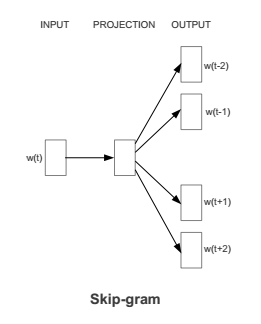
\includegraphics[width=\textwidth]{images/fig-2-sg}
    \caption{Modelo Skipgram}
    \label{fig:sg}
  \end{subfigure}

  \caption{Esquemas de word2vec}
\end{figure}

En los dos casos la probabilidad se modela utilizando exclusivamente un softmax jerárquico, como el
propuesto por Morin y Bengio en~\cite{MorinBengio2005}, con el fin de mejorar la eficiencia. Estos
dos nuevos modelos logran, por lo tanto, mejorar los resultados en la tarea de analogías a un costo
computacional significativamente menor que el de entrenar una RNN completa.

Cabe notar que, mientras que el autor lo plantea como la utilización de una red neuronal de una
única capa, también se puede ver directamente como una regresión logística multinomial, por lo que
el modelo se está simplificando enormemente con la finalidad de mejorar la eficiencia computacional,
en especial cuando se lo compara con modelos basados en RNNs. Dado el \textit{trade-off} que existe
entre la complejidad de los modelos estadísticos y la cantidad de datos que éstos pueden procesar,
este punto ubica a la propuesta de Mikolov como un modelo simple que requiere de muchos datos. De
hecho, en las pruebas que realiza el autor se utilizan corpus de texto del orden de los miles de
millones de palabras y, cuanto más aumenta el tamaño del mismo, mejores resultados obtiene.

En~\cite{Mikolov2013c}, Mikolov cierra su trabajo en representaciones vectoriales de palabras
presentando extensiones sobre el modelo Skipgram. El artículo comienza formalizando el modelo: se
presenta la función objetivo, que previamente había obviado, y se detalla la utilización del softmax
jerárquico. Luego se presenta una alternativa a esta última técnica que logra mejorar
significativamente los resultados, basada en \textit{Noise-contrastive Estimation} (NCE), propuesta
inicialmente por Gutmann y Hyyvärinen~\cite{Gutmann2012} y aplicada por Mnih y Teh para modelado de
lenguaje~\cite{MnihTeh2012}. Esta técnica, que denomina \textit{negative sampling} (NS), se basa en
generar ejemplos negativos de uso del lenguaje: esto es, además de utilizar el texto proveniente del
corpus de entrenamiento, se genera texto aleatorio, bajo la premisa de que será inválido
gramaticalmente, como ejemplo de mal uso del lenguaje.

El autor también presenta una serie de heurísticas para el procesamiento del corpus, como la
realización de \textit{subsampling} de palabras muy frecuentes (i.e.\ ignora aleatoriamente palabras que
son demasiado comunes en el corpus) y la eliminación de palabras muy raras, que mejoran aún más los
resultados.

Por último, junto a la publicación de este artículo, Mikolov presenta un nuevo conjunto de pruebas
mucho más extenso, que abarca tanto casos sintácticos como semánticos. También hace pública su
implementación de los modelos CBOW y Skipgram, bajo una herramienta denominada
\texttt{word2vec}. Este punto no es de menor importancia, porque contribuyó a aumentar el interés en
el tema, en especial entre el público amateur, y permitió reproducir y comparar los resultados con
distintos métodos de manera más correcta desde un punto de vista metodológico.


\section{Modelos Híbridos}

Los dos tipos de representaciones vectoriales descritos tienen mucha literatura detrás, pero al
haber surgido independientemente, carecían de comparaciones sistemáticas y completas entre ellos. La
primera de estas evaluaciones se realiza en~\cite{Baroni2014}.

En este artículo, los autores reúnen catorce conjuntos de pruebas utilizados por la comunidad para
los problemas de similitud entre palabras, analogías, y otros. Someten a estas pruebas a modelos
estadísticos (modelos basados en contar, como los llama el autor) y a modelos neuronales (modelos
basados en predecir). Para los primeros utiliza vectores construidos con la herramienta
\texttt{DISSECT}~\cite{Dinu2013}, basados principalmente en esquemas PMI con reducción de
dimensionalidad con SVD\@. Para los segundos utiliza la herramienta provista por Mikolov
en~\cite{Mikolov2013c}, \texttt{word2vec}.

Los resultados que obtienen los autores presentan a los modelos neuronales como grandes ganadores,
donde obtienen mejores resultados en todas las pruebas realizadas. Esta conclusión lleva a la
comunidad a investigar qué es lo que hace mejores a los métodos neuronales por sobre los
estadísticos.

Siguiendo esta línea de pensamiento, en~\cite{Levy2015} el autor busca identificar qué es lo que
hace que Skipgram con Negative Sampling (SGNS) funcione tanto mejor que un modelo PPMI que utiliza
SVD\@. Los resultados a los que llega, sin embargo, son contradictorios con los de Baroni. Plantea
que la diferencia entre la performance de ambos métodos se debe a que SGNS tiene una ventaja por
utilizar, además del modelo básico, una serie de heurísticas en el preprocesamiento del corpus y el
posprocesamiento de los vectores que mejoran drásticamente los resultados.

De esta forma, Levy identifica una serie de nueve heurísticas de uno y otro modelo, que los
considerará hiperparámetros, y los adapta para ambos esquemas. Además de hacer esto, entrena todos
los vectores utilizando exactamente el mismo corpus de datos (punto que no hizo Baroni, pues utilizó
vectores preentrenados descargados de Internet) y compara contra el mismo conjunto de pruebas. Así,
utilizando una metodología más robusta que en el estudio anterior, llega a que los resultados de los
modelos estadísticos y los modelos neuronales son prácticamente equivalentes, con los primeros con
una leve ventaja. De todos modos, el autor resalta que SGNS es mucho más eficiente
computacionalmente, lo que le permite utilizar más datos.


Más allá de las comparaciones, los dos enfoques anteriores no son necesariamente
ortogonales. En~\cite{Levy2014a} se muestra que SGNS está en realidad siguiendo un esquema muy
similar a los enfoques estadísticos, donde se realiza una factorización implícita de una matriz
SSPMI\@: esto es, una matriz PPMI donde la medida de asociación es $f(v_i, v_j) = \max(PMI(v_i, v_j)
- \log(k), 0)$, con $k$ un hiperparámetro del modelo. Este resultado es muy importante, pues conecta
directamente dos enfoques históricamente independientes. El autor plantea que la ventaja que SGNS
tiene sobre la matriz PPMI estándar se da en que su factorización está ponderada de modo de no dar
demasiada importancia a las palabras más comunes, una de las debilidades principales de la métrica
PPMI\@.


Siguiendo estos resultados, han surgido diversos métodos que plantean un esquema híbrido, donde se
busca hacer explícita la tarea de aprendizaje que se realiza, basándose en las lecciones aprendidas
de los enfoques ya presentados. Uno de estos métodos es GloVe, presentado en~\cite{Pennington2014},
donde los autores construyen una matriz $A$, similar a la matriz de asociación de los modelos
estadísticos, donde la función de asociación busca explícitamente quitar peso a las palabras más
frecuentes y no sobrerrepresentar a las muy poco frecuentes. Luego obtiene representaciones
vectoriales de baja dimensionalidad minimizando una función de costo asociada los vectores de
palabras y la matriz de coocurrencia, siguiendo un método iterativo que lo hace computacionalmente
más eficiente que SVD\@. Los resultados que obtienen los autores son superiores a los obtenidos por
SGNS en el conjunto de pruebas provisto por Mikolov\footnote{Cabe notar que en~\cite{Levy2015} no se
logra reproducir este resultado, aunque aun así es un método muy competitivo.}.


Los modelos estadísticos, neuronales e híbridos han resultado bastante similares en cuanto a los
resultados obtenidos. Reconociendo este punto, la comunidad se está centrando en modelos híbridos
que aprovechen las lecciones aprendidas por los tres enfoques, buscando nuevas métricas de
asociación (definiendo matrices de asociación explícitamente) y nuevas formas de factorizarlas (ya
sea con variantes de SVD, o con métodos iterativos).


\section{Evaluación y Estado del Arte}

Hasta ahora se presentaron distintos enfoques para la construcción de representaciones vectoriales,
pero no se ha detallado qué entendemos por estado del arte: esto es, cuándo consideramos que una
representación es mejor que otra, y cómo las comparamos.

Es posible comparar las representaciones de forma implícita y explícita. La primera implica evaluar
los cambios en la performance en un algoritmo de aprendizaje automático donde se usan; esto es, como
parte de una solución de un problema de PLN más grande. La segunda refiere a evaluar directamente la
calidad de los vectores obtenidos mediante alguna tarea de PLN desarrollada específicamente para el
caso.

Para la evaluación explícita, el objetivo es diseñar un experimento cuyo resultado esté, en la
medida de lo posible, correlacionado a la calidad de una solución de PLN de mayor porte cuando se
utilizan estas representaciones. Esto permite optimizar una métrica más definida y más fácil de
calcular. Por ejemplo, si se está construyendo una solución para el procesamiento automático del
habla (ASR), y se supiera que representaciones que funcionan mejor en la tarea de analogías mejoran
el resultado final, sería mucho más fácil y eficiente probar distintos hiperparámetros y modelos
evaluando con esa métrica, que entrenar todo un modelo de ASR de principio a fin para evaluar si los
vectores produjeron mejores resultados\footnote{Esto es particularmente problemático para los
vectores de palabras, pues suelen ser el primer componente en una solución PLN.}. En especial porque
en un modelo complejo, pueden haber varios componentes que afecten la calidad final de la solución,
por lo que no se sabrá si fueron los vectores los que mejoraron los resultados o no.

De todos modos, esta correlación entre la evaluación explícita e implícita de representaciones
vectoriales por lo general no se puede probar, y es una suposición que se toma cuando se realiza una
evaluación explícita.


En la literatura se han usado muchas tareas para la evaluación explícita de vectores, algunas de las
cuales ya han sido mencionadas brevemente. Una de las más antiguas es la tarea de similitud y
relación entre palabras, que busca decidir si una palabra es sustituible por otra en un contexto
dado. Para esto, se construye un conjunto de pruebas compuesto por pares de palabras y un puntaje,
determinado por un grupo de humanos, de qué tan similares son dichas palabras. El objetivo es
obtener un buen nivel de correlación entre los puntajes de los pares de palabras y las
distancias\footnote{Es usual utilizar la distancia euclídea o la distancia coseno.} en el espacio de
vectores, medida utilizando la correlación de Spearman. Distinguimos también entre similitud, donde
se mide relaciones más fuertes, como la sinonimia y la hiponimia, de la relación
(\textit{relatedness} en la literatura), donde se incluyen relaciones más amplias, posiblemente
temáticas.

Existen muchos conjuntos de prueba para esta tarea. Uno de los más utilizados es
WordSim353~\cite{Finkelstein2002}, compuesta de 353 pares de palabras, diferenciados entre relación
y similitud. También muy populares están MEN~\cite{Bruni2012}, compuesto de 1000 pares de palabras,
SimLex999~\cite{Hill2014}, y Mechanical Turk~\cite{Radinsky2011}.

Otra alternativa que ha surgido recientemente para el estudio de regularidades lingüísticas de
representaciones vectoriales es la tarea de analogías, propuesta inicialmente por Mikolov
en~\cite{Mikolov2013a}. En este escenario, se cuenta con dos pares de palabras que mantienen una
misma relación (sintáctica o semántica) y se busca determinar la cuarta palabra a partir de las
anteriores tres. Por ejemplo, si se cuenta con los pares de palabras \textit{correr} y
\textit{corriendo}, \textit{jugar} y \textit{jugando}, el objetivo es, a partir de los vectores de
\textit{correr}, \textit{corriendo} y \textit{jugar}, lograr recuperar la cuarta palabra,
\textit{jugando}.

Para esto Mikolov originalmente propone en~\cite{Mikolov2013a} utilizar la función \textsc{3CosAdd}
para recuperar la cuarta palabra, definida como:

\[
  {\arg \max}_{b' \in V} \cos(b', b - a + a')
\]

Donde los pares de analogías son $(a, a')$ y $(b, b')$ y $\cos$ la similitud coseno. Sin embargo,
en~\cite{Levy2014b}, Levy prueba que una mejor función para la recuperación de analogías es
\textsc{3CosMul}, definida como:

\[
  {\arg \max}_{b' \in V} \frac{\cos(b', b) \cos(b', a')}{\cos(b', a) + \epsilon}
\]

Donde $\epsilon$ es un valor muy pequeño (e.g.\ $\epsilon = 0.001$) utilizado para evitar la
división entre cero.

Mikolov introdujo inicialmente un conjunto de 8000 analogías exclusivamente sintácticas
en~\cite{Mikolov2013a}, con relaciones como plurales y conjugaciones verbales. Luego introduce
en~\cite{Mikolov2013b} un conjunto de analogías más amplio que cuenta con cerca de 20000 analogías,
tanto sintácticas como semánticas.

Existen también otras tareas que se han utilizado, aunque en menor medida, para la evaluación
explícita de vectores, como la utilización del TOEFL (\textit{Test of English as Foreign Language},
una prueba utilizada para medir el conocimiento de inglés) de~\cite{LandauerDumais1997}, la
categorización de conceptos de~\cite{Almuhareb2006}, y la preferencia de selección
de~\cite{Pado2007}.


En cuanto a evaluación implícita de las representaciones vectoriales, y cómo se relaciona con los
resultados de la evaluación explícita, no existe mucho trabajo en la literatura. Un trabajo
preliminar que toca superficialmente este punto es~\cite{Qu2015}, donde los autores utilizan
distintos modelos vectoriales (SGNS, GloVe, los vectores de Collobert y Weston, y Brown Clusters)
como features de algoritmos de clasificación secuencial (principalmente CRFs, para resolver los
problemas de POS tagging y NER). Llegan a que, al usar distintas representaciones bajo este esquema
(donde los vectores son una feature más), los resultados mejoran de manera muy similar para los
distintos modelos: esto es, se obtiene la misma ganancia utilizando Brown Clusters (que genera una
representación más rudimentaria) que SGNS\@.

Existe también un poco de escepticismo por parte de algunos investigadores en el área respecto a qué
beneficios proveen los vectores de palabras. Edward Grefenstette escribe~\cite{Reddit2016} que las
representaciones vectoriales parecen ser principalmente una forma de aprendizaje por transferencia,
donde se entrena con la tarea de analogías o similitud entre palabras para resolver una tarea más
compleja. Plantea que esto es beneficioso cuando se trabaja con corpus de entrenamiento demasiado
chicos, pues ayuda a la generalización, pero que no son necesarios e incluso pueden perjudicar la
performance cuando se tienen suficientes datos.

Otro caso que fortalece este argumento es el hecho que en~\cite{CollobertWeston2008} se obtienen muy
buenos resultados en el etiquetado de roles semánticos, pero los vectores son inferiores en la tarea
de analogías (como muestra~\cite{Mikolov2013a}). Esto, de todos modos, puede resultar del hecho que
los autores ajustan los valores de los vectores en la medida que entrenan con las otras tareas.

Estos puntos son importantes y requieren de mayor investigación, pues determinan qué tanto es
necesario buscar nuevos y mejores modelos vectoriales. Es posible, por ejemplo, que pequeñas
diferencias en los resultados de evaluación explícita sean compensados por el modelo que los usa,
como pasa con los Brown Clusters en~\cite{Qu2015}. En este caso, se podría incluso utilizar un
corpus más chico para entrenar las representaciones, o vectores más simples.


De todos modos, en el presente proyecto se estará realizando una evaluación puramente explícita de
los modelos vectoriales entrenados, por varias razones. En primer lugar, el objetivo es realizar una
investigación del comportamiento de representaciones vectoriales en general, no de un problema de
PLN particular. Segundo, porque no hay un estándar en evaluación implícita con el que se pueda
comparar los resultados, ni que sean una aplicación directa de vectores de palabras. Tercero, porque
realizar una evaluación implícita sería mucho más costoso computacional y metodológicamente, lo que
nos impediría probar con una gran variedad de modelos. Y por último, porque las tareas con las que
se estarán evaluando, analogías y similitud de palabras, entre otros, tienen de por sí aplicaciones
directas que son de gran utilidad.


En cuanto a los modelos vectoriales que se evaluarán, se decidió optar por un representante de cada
enfoque: Skipgram y CBOW como modelos neuronales, una matriz PPMI con SVD como modelo estadístico, y
GloVe como modelo híbrido. Se eligen estos cuatro modelos por ser los que consiguen los mejores
resultados en las tareas de analogías y similitud de palabras en la literatura en inglés, evitando
así sesgarnos a un esquema de representación vectorial particular, y pudiendo evaluar si alguno de
ellos tiene un comportamiento particular para el idioma español.
